%%%%%%%%%%%%%%%%%%%%%%%%%%%%%%%%%%%%%%%%%
% Structured General Purpose Assignment
% LaTeX Template
%
% This template has been downloaded from:
% http://www.latextemplates.com
%
% Original author:
% Ted Pavlic (http://www.tedpavlic.com)
%
% Note:
% The \lipsum[#] commands throughout this template generate dummy text
% to fill the template out. These commands should all be removed when 
% writing assignment content.
%
%%%%%%%%%%%%%%%%%%%%%%%%%%%%%%%%%%%%%%%%%

%----------------------------------------------------------------------------------------
%	PACKAGES AND OTHER DOCUMENT CONFIGURATIONS
%----------------------------------------------------------------------------------------

\documentclass{article}

\usepackage{fancyhdr} % Required for custom headers
\usepackage{lastpage} % Required to determine the last page for the footer
\usepackage{extramarks} % Required for headers and footers
\usepackage{graphicx} % Required to insert images
\usepackage{caption}
\usepackage{float}
\usepackage{url}
\usepackage{subcaption}


% Margins
\topmargin=-0.45in
\evensidemargin=0in
\oddsidemargin=0in
\textwidth=6.5in
\textheight=9.0in
\headsep=0.25in 


\linespread{1.1} % Line spacing

% Set up the header and footer
\pagestyle{fancy}
\lhead{\hmwkAuthorName} % Top left header
\chead{\hmwkClass\ \hmwkTitle} % Top center header
\rhead{\firstxmark} % Top right header
\lfoot{\lastxmark} % Bottom left footer
\cfoot{} % Bottom center footer
\rfoot{Page\ \thepage\ of\ \pageref{LastPage}} % Bottom right footer
\renewcommand\headrulewidth{0.4pt} % Size of the header rule
\renewcommand\footrulewidth{0.4pt} % Size of the footer rule

\setlength\parindent{0pt} % Removes all indentation from paragraphs

%----------------------------------------------------------------------------------------
%	DOCUMENT STRUCTURE COMMANDS
%	Skip this unless you know what you're doing
%----------------------------------------------------------------------------------------

% Header and footer for when a page split occurs within a problem environment
\newcommand{\enterProblemHeader}[1]{
\nobreak\extramarks{#1}{#1 continued on next page\ldots}\nobreak
\nobreak\extramarks{#1 (continued)}{#1 continued on next page\ldots}\nobreak
}

% Header and footer for when a page split occurs between problem environments
\newcommand{\exitProblemHeader}[1]{
\nobreak\extramarks{#1 (continued)}{#1 continued on next page\ldots}\nobreak
\nobreak\extramarks{#1}{}\nobreak
}

\setcounter{secnumdepth}{0} % Removes default section numbers
\newcounter{homeworkProblemCounter} % Creates a counter to keep track of the number of problems

\newcommand{\homeworkProblemName}{}
\newenvironment{homeworkProblem}[1][Problem \arabic{homeworkProblemCounter}]{ % Makes a new environment called homeworkProblem which takes 1 argument (custom name) but the default is "Problem #"
\stepcounter{homeworkProblemCounter} % Increase counter for number of problems
\renewcommand{\homeworkProblemName}{#1} % Assign \homeworkProblemName the name of the problem
\section{\homeworkProblemName} % Make a section in the document with the custom problem count
\enterProblemHeader{\homeworkProblemName} % Header and footer within the environment
}{
\exitProblemHeader{\homeworkProblemName} % Header and footer after the environment
}

\newcommand{\problemAnswer}[1]{ % Defines the problem answer command with the content as the only argument
\noindent\framebox[\columnwidth][c]{\begin{minipage}{0.98\columnwidth}#1\end{minipage}} % Makes the box around the problem answer and puts the content inside
}

\newcommand{\homeworkSectionName}{}
\newenvironment{homeworkSection}[1]{ % New environment for sections within homework problems, takes 1 argument - the name of the section
\renewcommand{\homeworkSectionName}{#1} % Assign \homeworkSectionName to the name of the section from the environment argument
\subsection{\homeworkSectionName} % Make a subsection with the custom name of the subsection
\enterProblemHeader{\homeworkProblemName\ [\homeworkSectionName]} % Header and footer within the environment
}{
\enterProblemHeader{\homeworkProblemName} % Header and footer after the environment
}
   
%----------------------------------------------------------------------------------------
%	NAME AND CLASS SECTION
%----------------------------------------------------------------------------------------

\newcommand{\hmwkTitle}{"Where Have I Been?" - Languages Comparison} % Assignment title
\newcommand{\hmwkDueDate}{Friday,\ April\ 11,\ 2014} % Due date
\newcommand{\hmwkClass}{CS\ 22510} % Course/class
\newcommand{\hmwkAuthorName}{James Euesden - jee22} % Your name

%----------------------------------------------------------------------------------------
%	TITLE PAGE
%----------------------------------------------------------------------------------------

\title{
\vspace{2in}
\textmd{\textbf{\hmwkClass:\ \hmwkTitle}}\\
\normalsize\vspace{0.1in}\small{Due\ on\ \hmwkDueDate}\\
\vspace{3in}
}

\author{\textbf{\hmwkAuthorName}}
\date{} % Insert date here if you want it to appear below your name

%----------------------------------------------------------------------------------------

\setlength\parindent{24pt}

\begin{document}

\maketitle

%----------------------------------------------------------------------------------------
%	TABLE OF CONTENTS
%----------------------------------------------------------------------------------------

%\setcounter{tocdepth}{1} % Uncomment this line if you don't want subsections listed in the ToC

\newpage
\tableofcontents
\newpage

%----------------------------------------------------------------------------------------
%	INTRODUCTION
%----------------------------------------------------------------------------------------

% To have just one problem per page, simply put a \clearpage after each problem

\section{Introduction}
This document is the second part (Assignment 2\cite{assignment}) of the "Where have I been?" assignment. In this report, I will discuss the languages and my experiences with them. While the first part (Assignment 1) was about the programming for GPS Processing, this is about the differences and similarities between them. What I found useful, or difficult, between the languages, any libraries I may have chosen to use, and what language I felt was best suited to the task.


%----------------------------------------------------------------------------------------
%	LANGUAGE COMPARISONS
%----------------------------------------------------------------------------------------

\section{Language Comparisons}

The amount of code between each language was rather similar. I used GitHub to keep track of my code and the versions of it as I completed part one of the assignment. One of the benefits of doing this was that it provided a great break down of how much percentage of the repo was taken up by the different components (screenshot taken before this document was added to the repository):

\begin{figure}[h!]
  \caption{The percentage of languages on the GitHub repo for part 1.}
  \centering
    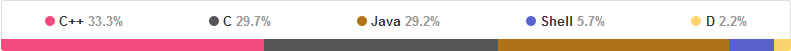
\includegraphics[width=1\textwidth]{img/percentages}
\end{figure}

The figure shows that the amount of code for each language that I wrote was very similar. I feel the reason C++ has more code than the other two may be due to each class having a Constructor, a Destructor and a Copy Constructor, whether they were used or not. With this in mind, it should be apparent that my writing of the application in each language was very similar, and while one particular section may take more code than another, that same language may do something much simpler than in another too.

An example would be the file operations in Java vs C, where it takes more for C to handle getting the data out of the file and char arrays than in Java. Opposite to this, my C program handles date and time much easier and with less code than that used in Java for the most part. Overall, I found the simplicity of C and C++ help me in writing the code in the most simplest way I could think of. A huge benefit over Java, where I sometimes felt I was writing bloated code that was unnecessary (and later refactored out).

\subsection{File Operations}

In all three languages, the file input and output was relatively simple and similar. With Java, I had a slight difference in that on every update of a timestamp I output the XML into a StringBuilder, and then output the full String at the very end of the application. While with the C and C++, I output directly to the file when a timestamp was updated. This was made very easy through the use of pointers to the FILE, and keeping a reference to the class for the file operations.

\subsection{Data Accessibility \& Manipulation}

With Java and C++ having objects rather than simple source files with functions and variables, it was fantastic to be able to put a variable as private, and restrict access to it from outside of the class except through the defined use of getters and setters. While something similar can be done

\subsection{Date \& Time}

For both C and C++ I used the 'time' library\cite{time}, and for Java used the Calendar class. I found the Calendar class cumbersome to use and in some ways hindered my programming. On the otherhand, using the time library was perfect for checking the timestamps between sentences, comparing them, creating new timestamps from sentence data and even updating a timestamp with new sentence data without a date. 

When programming in Java and using Calendar, making a new time with the date and time provided by a sentence was fine. When it came to updating a time without a provided date, it became much more difficult to do. My method for handling this in all three languages was similar. Just use the most recent date provided (potential pitfall for the application's future use where the time passes 00:00. This could be rectified in a future edition). 

This was simple to do in C and C++, with simply turning the time\_t struct back into a tm struct, updating the values and then using mktime() to get it back to time\_t. While the process with Calendar is similar, I found that I had trouble getting the time to be correct, with milliseconds assigned randomly, and needing to use .clone() to get correct values for the date.




%-------------------------------------------- Compare/Contrast. Amount of code written, the clarity of code, any features that helped/hindered the representation of my solution.



%----------------------------------------------------------------------------------------
%	LIBRARIES
%----------------------------------------------------------------------------------------

\section{Libraries}

I chose not to use any libraries outside of those provided with the standard API of the native languages. Below are those libraries that I could have used, why they could have been useful, and why I didn't use them.

\subsection{NMEA parsing}
For all three languages there are libraries that I could have used in order to parse the NMEA sentences into data, without me having to dissect them myself and extract the data\cite{nmeajava}\cite{nmeacplusplus}. However, I chose not to use any of these. My main reason for this is that I wanted to understand the sentences myself, and to only extract the data I wanted and then discard them, rather than extract all data from the sentences. On a larger project that intended to use the majority of data from the NMEA sentences, I would look into using one of these open source libraries to save time. For my own assignment in my own work, I felt that it was acceptable to not use these.

\subsection{C++: Boost}
There is a library for C++ called Boost\cite{boost}. This library provides many useful functions for C++ that aren't in the native language. A number of these could be have been useful for manipulating strings, and saved me time and code. However, as with the NMEA 0813 sentences, for an assignment of this size I would rather use my own code and work through the problem to better my understanding of C++. Boost is a useful library that I will remember for future, larger, projects where their functions may be invaluable in saving me time and effort.

\subsection{Java: DocumentBuilder \& XML Builders}
While not an additional library, Java has the use for classes such as DocumentBuilder, which can XML tag a file (UTF-8) for us. Again, I chose not to use this, and provided my own methods for putting tags around the data. This is partially because of tags such as "<wpt lat="" lon=""> where it is a tag built up of multiple components I found easier to do myself, and also because of the size and amount of XML tags being output. If the applications were required to output a larger variety of XML tags, I may have found it useful to find XML Builders. For what the problem consisted of, I felt it was easy enough to do it myself, and to further my understanding of building XML files in my programming.

%-------------------------------------------- What Libraries could I have used? How could they have helped?

%----------------------------------------------------------------------------------------
%	SUITABILITY
%----------------------------------------------------------------------------------------

\section{Suitability}

In terms of what language is best suited for writing this application, I would say that a lot of it comes down to personal opinion. I found all three languages had their challenges or parts that aided me, and so each of them is relatively suitable for this process. 

However, out of all of them I felt that C++  was the most suitable for my implementation. My justification for this is that I found it the easiest and quickest to write in. The functions are all relatively simplistic, it has the simplicity of C, while providing the bonuses of Object Oriented programming like in Java. The fact that C++ has access to it's own libraries and functions, while also having access to those provided in C, made C++ an joy to write the application in.

%-------------------------------------------- Which Language was best for the task set, and why?



%----------------------------------------------------------------------------------------
%	CONCLUSION
%----------------------------------------------------------------------------------------
\clearpage

\section{Conclusion}


%----------------------------------------------------------------------------------------
\clearpage

%----------------------------------------------------------------------------------------
%	REFERENCES
%----------------------------------------------------------------------------------------

\begin{thebibliography}{1}

%---- \bibitem{assignment} D. Price and F. Long, "For those in Peril on the Sea.", CS23710 Assessed Assignment 2013-2014, November 11 2013

%---- \bibitem{ctime} ctime - cppreference, {\em cppreference},[online], http://en.cppreference.com/w/c/chrono/ctime (Accessed:10/12/2013)

\end{thebibliography}


\end{document}


